% Projet POWER : XGBoost, LightGBM et CatBoost face à la prévision RTE, et le tableau de bord
% Compiler avec pdfLaTeX (Overleaf) ou tectonic, avec le dossier figures/.
% Version courte : le détail des idées est dans journal/pistes_et_comparaison.md
\documentclass[aspectratio=169,10pt]{beamer}

\usepackage[utf8]{inputenc}
\usepackage[T1]{fontenc}
\usepackage[french]{babel}
\usepackage{helvet}
\renewcommand{\familydefault}{\sfdefault}
\usepackage{graphicx}
\usepackage{booktabs}
\usepackage{amssymb}
\usepackage{tikz}
\usetikzlibrary{positioning,arrows.meta,decorations.pathreplacing}
% faire apparaître un élément TikZ à une étape donnée
\tikzset{invisible/.style={opacity=0},
  visible on/.style={alt={#1{}{invisible}}},
  alt/.code args={<#1>#2#3}{\alt<#1>{\pgfkeysalso{#2}}{\pgfkeysalso{#3}}}}

% ---------- Couleurs du projet ----------
\definecolor{bleuPOWER}{RGB}{51,51,170}
\definecolor{grisBande}{RGB}{140,140,140}
\definecolor{grisTexte}{RGB}{90,90,100}
\definecolor{orangeRTE}{RGB}{217,105,43}
\definecolor{vertBon}{RGB}{40,120,60}
\definecolor{fondCarte}{RGB}{238,238,248}
% couleurs du planning
\definecolor{ganttFait}{RGB}{46,140,80}
\definecolor{ganttCours}{RGB}{51,51,170}
\definecolor{ganttVenir}{RGB}{205,205,215}
\definecolor{ganttJalon}{RGB}{200,40,40}

% ---------- Style : bandeau gris, titre sur fond bleu, numéro en haut à droite ----------
\setbeamertemplate{navigation symbols}{}
\setbeamercolor{normal text}{fg=black,bg=white}
\setbeamercolor{structure}{fg=bleuPOWER}
\setbeamercolor{alerted text}{fg=bleuPOWER}
\setbeamerfont{frametitle}{size=\Large}
\setbeamertemplate{itemize item}{\color{bleuPOWER}$\blacksquare$}
\setbeamertemplate{itemize subitem}{\color{bleuPOWER}--}
\setbeamercovered{invisible}

\setbeamertemplate{frametitle}{%
  \vspace*{-0.2ex}%
  \begin{tikzpicture}[remember picture,overlay]
    \fill[grisBande] (current page.north west) rectangle ([yshift=-0.55cm]current page.north east);
    \fill[bleuPOWER] ([yshift=-0.55cm,xshift=0.3cm]current page.north west)
                     rectangle ([yshift=-1.55cm,xshift=-1.6cm]current page.north east);
    \fill[bleuPOWER] ([yshift=-0.75cm,xshift=-1.25cm]current page.north east)
                     rectangle ([yshift=-0.95cm,xshift=-1.05cm]current page.north east);
    \node[anchor=west,text=white,font=\Large] at ([yshift=-1.05cm,xshift=0.7cm]current page.north west)
         {\insertframetitle};
    \node[text=bleuPOWER,font=\small] at ([yshift=-1.3cm,xshift=-0.75cm]current page.north east)
         {\insertframenumber};
  \end{tikzpicture}%
  \vspace*{1.25cm}%
}

\newcommand{\source}[1]{\par\vfill{\scriptsize\color{grisTexte}#1}}
\newcommand{\bon}[1]{{\color{vertBon}\textbf{#1}}}
\newcommand{\rte}[1]{{\color{orangeRTE}\textbf{#1}}}
% une figure par modèle, qui apparaît à l'étape #1
\newcommand{\fig}[3]{\uncover<#1->{\centering\textbf{#2}\\[0.2em]
  \includegraphics[width=\linewidth,height=0.42\textheight,keepaspectratio]{#3}}}
% une cellule de tableau qui apparaît à l'étape #1
\newcommand{\pop}[2]{\uncover<#1->{#2}}
% une boîte du schéma du tableau de bord
\tikzset{boite/.style={draw=bleuPOWER,fill=fondCarte,rounded corners=2pt,thick,
  minimum width=3.6cm,minimum height=1.5cm,align=center,font=\small}}

% nom d'une personne dans une boîte
\newcommand{\qui}[1]{{\color{bleuPOWER}\bfseries #1}\\[0.15em]}
% lignes du planning : nom, rang, (début, fin en semaines), couleur, étape d'apparition
\newcommand{\ggroupe}[3]{\node[anchor=west,text=bleuPOWER,font=\scriptsize\bfseries,visible on=<#3->] at (-5,-#2) {#1};}
\newcommand{\gtache}[6]{%
  \node[anchor=west,visible on=<#6->] at (-4.8,-#2) {#1};
  \fill[#5,visible on=<#6->] (#3,-#2-0.38) rectangle (#4,-#2+0.38);}

\begin{document}

% =====================================================================
\begin{frame}[plain]
  \begin{tikzpicture}[remember picture,overlay]
    \fill[bleuPOWER] ([yshift=-1.4cm]current page.north west) rectangle ([yshift=-5.2cm]current page.north east);
    \node[anchor=west,text=white,font=\huge\bfseries] at ([yshift=-2.7cm,xshift=1cm]current page.north west)
         {Trois modèles face à RTE};
    \node[anchor=west,text=white,font=\large] at ([yshift=-3.7cm,xshift=1cm]current page.north west)
         {XGBoost, LightGBM, CatBoost, et le tableau de bord};
    \node[anchor=west,text=grisTexte,font=\normalsize] at ([yshift=-6.2cm,xshift=1cm]current page.north west)
         {Projet POWER $\cdot$ prévision de la consommation électrique en France};
    \node[anchor=west,text=grisTexte,font=\small] at ([yshift=-6.9cm,xshift=1cm]current page.north west)
         {Validation 2024 $\cdot$ novembre 2026};
  \end{tikzpicture}
\end{frame}

% =====================================================================
\begin{frame}{Qui a fait quoi}
  \centering
  \begin{tikzpicture}[
      tache/.style={draw=bleuPOWER,fill=fondCarte,rounded corners=2pt,thick,
                    minimum width=3.3cm,minimum height=1.3cm,align=center,font=\small},
      fleche/.style={-{Stealth[length=2.5mm]},thick,bleuPOWER}]
    \node[tache] (meteo) at (0,0) {\qui{Hugo}Météo : stations,\\Tempo, météo prévue};
    \node[tache,visible on=<2->] (lgbm) at (4.8,1.8) {\qui{Momo}LightGBM};
    \node[tache,visible on=<2->] (cat) at (4.8,0) {\qui{Maxime}CatBoost + SHAP};
    \node[tache,visible on=<2->] (xgb) at (4.8,-1.8) {\qui{Yassine}XGBoost};
    \node[tache,visible on=<3->] (dash) at (9.6,0) {\qui{Amine}Tableau de bord\\Streamlit};
    \foreach \m in {lgbm,cat,xgb} {
      \draw[fleche,visible on=<2->] (meteo.east) -- (\m.west);
      \draw[fleche,visible on=<3->] (\m.east) -- (dash.west);
    }
  \end{tikzpicture}

  \vspace{1.2em}
  \uncover<4->{\small Base de données commune (PostgreSQL) et règles communes : même découpage, même règle des 48\,h.}
\end{frame}

% =====================================================================
\begin{frame}{Le même cadre pour les trois modèles}
  \begin{columns}[T]
    \begin{column}{0.31\textwidth}
      \uncover<1->{%
      \textbf{Découpage dans le temps}
      \begin{itemize}
        \item Entraînement 2012-2023
        \item Validation 2024
        \item Test 2025 : une seule fois, à la fin
      \end{itemize}}
    \end{column}
    \begin{column}{0.31\textwidth}
      \uncover<2->{%
      \textbf{Règles}
      \begin{itemize}
        \item Rien de connu moins de 48\,h avant
        \item Prévision RTE jamais en entrée
        \item Tempo exclu
      \end{itemize}}
    \end{column}
    \begin{column}{0.31\textwidth}
      \uncover<3->{%
      \textbf{Contrôle}
      \begin{itemize}
        \item 8\,783 heures communes
        \item RTE et la méthode naïve ont le \bon{même score} chez les trois
        \item $\Rightarrow$ mêmes heures, mêmes données
      \end{itemize}}
    \end{column}
  \end{columns}
\end{frame}

% =====================================================================
\begin{frame}{Tempo : finalement retiré}
  \begin{columns}[T]
    \begin{column}{0.31\textwidth}\uncover<1->{\textbf{1. Historique incomplet}\\[0.3em]Rien avant septembre 2014}\end{column}
    \begin{column}{0.31\textwidth}\uncover<2->{\textbf{2. Déjà dans la météo}\\[0.3em]Couleur choisie d'après la température}\end{column}
    \begin{column}{0.31\textwidth}\uncover<3->{\textbf{3. Peu d'effet}\\[0.3em]Annoncée seulement la veille}\end{column}
  \end{columns}
  \vspace{1.4em}
  \centering
  \uncover<4->{%
  \begin{tabular}{lrrr}
    \toprule
    Version (LightGBM) & MAPE & MAE & Poids de Tempo \\
    \midrule
    Sans Tempo & 1,87\,\% & 952 MW & -- \\
    Tempo décalé de 48\,h & 1,85\,\% & 938 MW & \textbf{0,0\,\%} \\
    {\color{grisTexte}Tempo du jour (triche)} & {\color{grisTexte}1,82\,\%} & {\color{grisTexte}922 MW} & {\color{grisTexte}0,7\,\%} \\
    \bottomrule
  \end{tabular}}

  \vspace{1.2em}
  \uncover<5->{%
  \begin{block}{Décision}
    Le modèle ne s'en sert pas : on retire Tempo.
  \end{block}}
\end{frame}

% =====================================================================
\begin{frame}{Les scores sur la validation 2024}
  \centering
  \begin{tabular}{lrrrr}
    \toprule
     & \textbf{MAE} & \textbf{RMSE} & \textbf{MAPE} & \textbf{Biais} \\
    \midrule
    \rte{RTE J-1}            & 1\,428 MW & 1\,766 MW & 2,86\,\% & $-$1\,146 MW \\
    \pop{2}{\textbf{XGBoost}}  & \pop{2}{1\,254 MW} & \pop{2}{--} & \pop{2}{2,43\,\%} & \pop{2}{+838 MW} \\
    \pop{3}{\textbf{LightGBM}} & \pop{3}{\bon{800 MW}} & \pop{3}{1\,065 MW} & \pop{3}{\bon{1,58\,\%}} & \pop{3}{$-$127 MW} \\
    \pop{4}{\textbf{CatBoost}} & \pop{4}{--} & \pop{4}{\bon{968 MW}} & \pop{4}{--} & \pop{4}{$-$260 MW} \\
    \bottomrule
  \end{tabular}

  \vspace{1.2em}
  \begin{itemize}
    \item<5-> Les trois modèles \textbf{battent RTE} : XGBoost de 12\,\%, LightGBM de 44\,\% (MAE)
    \item<6-> Sur ce qui se compare : \textbf{CatBoost devant LightGBM} (RMSE), \textbf{LightGBM devant XGBoost} (MAE)
    \item<7-> XGBoost \textbf{surestime} (+838 MW) : c'est le score de LightGBM \emph{sans} \texttt{evt\_energie} (2,39\,\%, +782 MW)
  \end{itemize}
  \source{-- : indicateur non communiqué par le modèle. Le R$^2$ n'est pas comparé.}
\end{frame}

% =====================================================================
\begin{frame}{Une semaine d'hiver et une d'été}
  \begin{columns}[T]
    \begin{column}{0.33\textwidth}\fig{1}{XGBoost}{figures/xgboost_01_semaines.png}\end{column}
    \begin{column}{0.33\textwidth}\fig{2}{LightGBM}{figures/lightgbm_01_semaines.png}\end{column}
    \begin{column}{0.33\textwidth}\fig{3}{CatBoost}{figures/catboost_01_semaines.png}\end{column}
  \end{columns}
  \vspace{0.6em}
  \begin{itemize}
    \item<4-> \textbf{Été} : les trois collent au réel, \rte{RTE reste en dessous} l'après-midi
    \item<5-> \textbf{Hiver} : les trois manquent le froid des 9-10 janvier ; XGBoost surestime le 12
  \end{itemize}
\end{frame}

% =====================================================================
\begin{frame}{L'erreur selon l'heure}
  \begin{columns}[T]
    \begin{column}{0.33\textwidth}\fig{1}{XGBoost \small(MW)}{figures/xgboost_03_mae_par_heure.png}\end{column}
    \begin{column}{0.33\textwidth}\fig{2}{LightGBM \small(MW)}{figures/lightgbm_03_mae_par_heure.png}\end{column}
    \begin{column}{0.33\textwidth}\fig{3}{CatBoost \small(\%)}{figures/catboost_03_mape_par_heure.png}\end{column}
  \end{columns}
  \vspace{0.6em}
  \begin{itemize}
    \item<4-> Nos trois modèles : erreur \textbf{régulière} sur toute la journée
    \item<5-> RTE : \rte{pics à 0\,h, 13-16\,h et 20-21\,h}, presque parfait à 5\,h et 8\,h
    \item<6-> Même forme chez les trois $\Rightarrow$ le biais vient de RTE, pas de nos codes
  \end{itemize}
\end{frame}

% =====================================================================
\begin{frame}{SHAP : expliquer chaque prévision, heure par heure}
  \begin{columns}[T]
    \begin{column}{0.56\textwidth}
      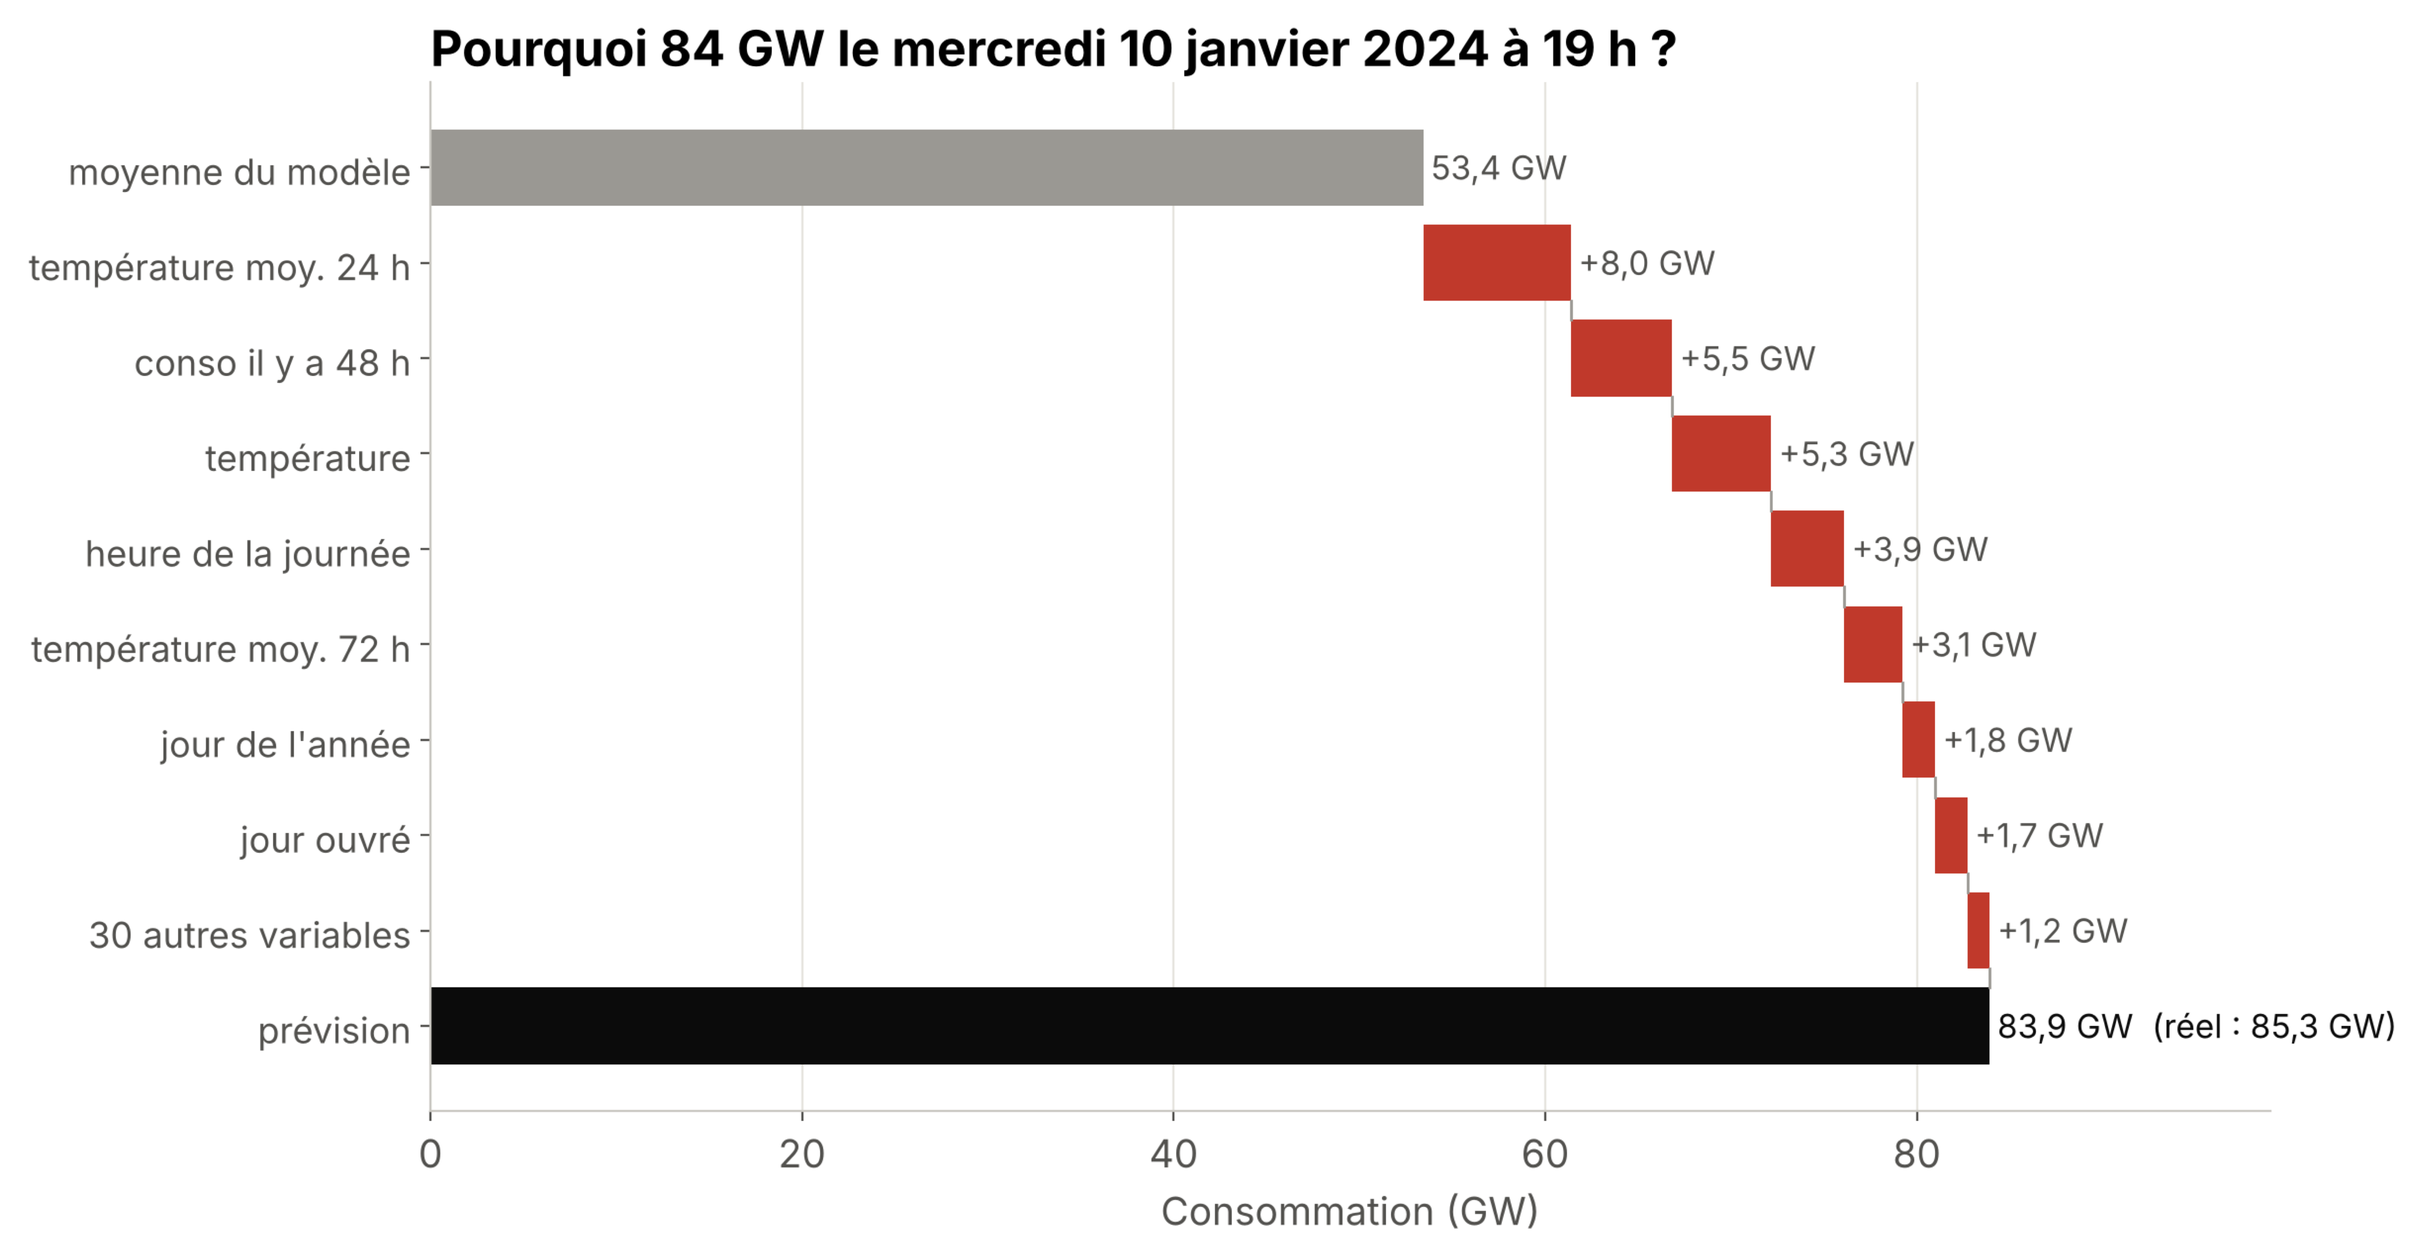
\includegraphics[width=\linewidth,height=0.5\textheight,keepaspectratio]{figures/shap_cascade_10janvier.png}\\
      {\scriptsize\color{grisTexte}CatBoost, 10 janvier 2024 à 19\,h : 0,6\,$^{\circ}$C, moyenne sur 24\,h $-$0,4\,$^{\circ}$C.}
    \end{column}
    \begin{column}{0.42\textwidth}\small
      \uncover<2->{%
      \textbf{Comment lire}
      \begin{itemize}
        \item On part de la moyenne du modèle : \textbf{53 GW}
        \item Chaque variable ajoute ou retire sa part
        \item La somme donne la prévision : \textbf{84 GW} (réel 85)
      \end{itemize}}
      \vspace{0.5em}
      \uncover<3->{%
      \textbf{Ce que ça apporte}
      \begin{itemize}
        \item Le \textbf{sens} de l'effet : ici, le froid ajoute 16 GW
        \item Une explication pour \textbf{chaque heure}, utile au tableau de bord
      \end{itemize}}
    \end{column}
  \end{columns}
  \vspace{0.2em}
  \uncover<4->{%
  \begin{block}{Attention}
    SHAP explique le \textbf{modèle}, pas la physique : les +5,5 GW de la conso d'il y a 48\,h viennent surtout du froid qui durait déjà.
  \end{block}}
\end{frame}

% =====================================================================
\begin{frame}{Sur quoi chaque modèle s'appuie}
  \begin{columns}[T]
    \begin{column}{0.33\textwidth}\fig{1}{XGBoost \small(gain)}{figures/xgboost_04_importance.png}\end{column}
    \begin{column}{0.33\textwidth}\fig{2}{LightGBM \small(SHAP)}{figures/lightgbm_04_importance.png}\end{column}
    \begin{column}{0.33\textwidth}\fig{3}{CatBoost \small(SHAP)}{figures/catboost_04_importance.png}\end{column}
  \end{columns}
  \vspace{0.6em}
  \begin{itemize}
    \item<4-> Les trois s'appuient sur le \textbf{passé de la conso}, le calendrier et la température ; XGBoost utilise \texttt{est\_heure\_ete} (20\,\%) comme indicateur de saison
    \item<5-> LightGBM et CatBoost : \textbf{températures lissées} sur 24\,h et \texttt{evt\_energie} pèsent lourd ; XGBoost n'a ni l'une ni l'autre
    \item<6-> XGBoost mesure le \emph{gain}, qui gonfle le passé : à refaire en SHAP pour comparer
  \end{itemize}
\end{frame}

% =====================================================================
\begin{frame}{Importance native ou SHAP : pas le même classement}
  \begin{columns}[T]
    \begin{column}{0.56\textwidth}
      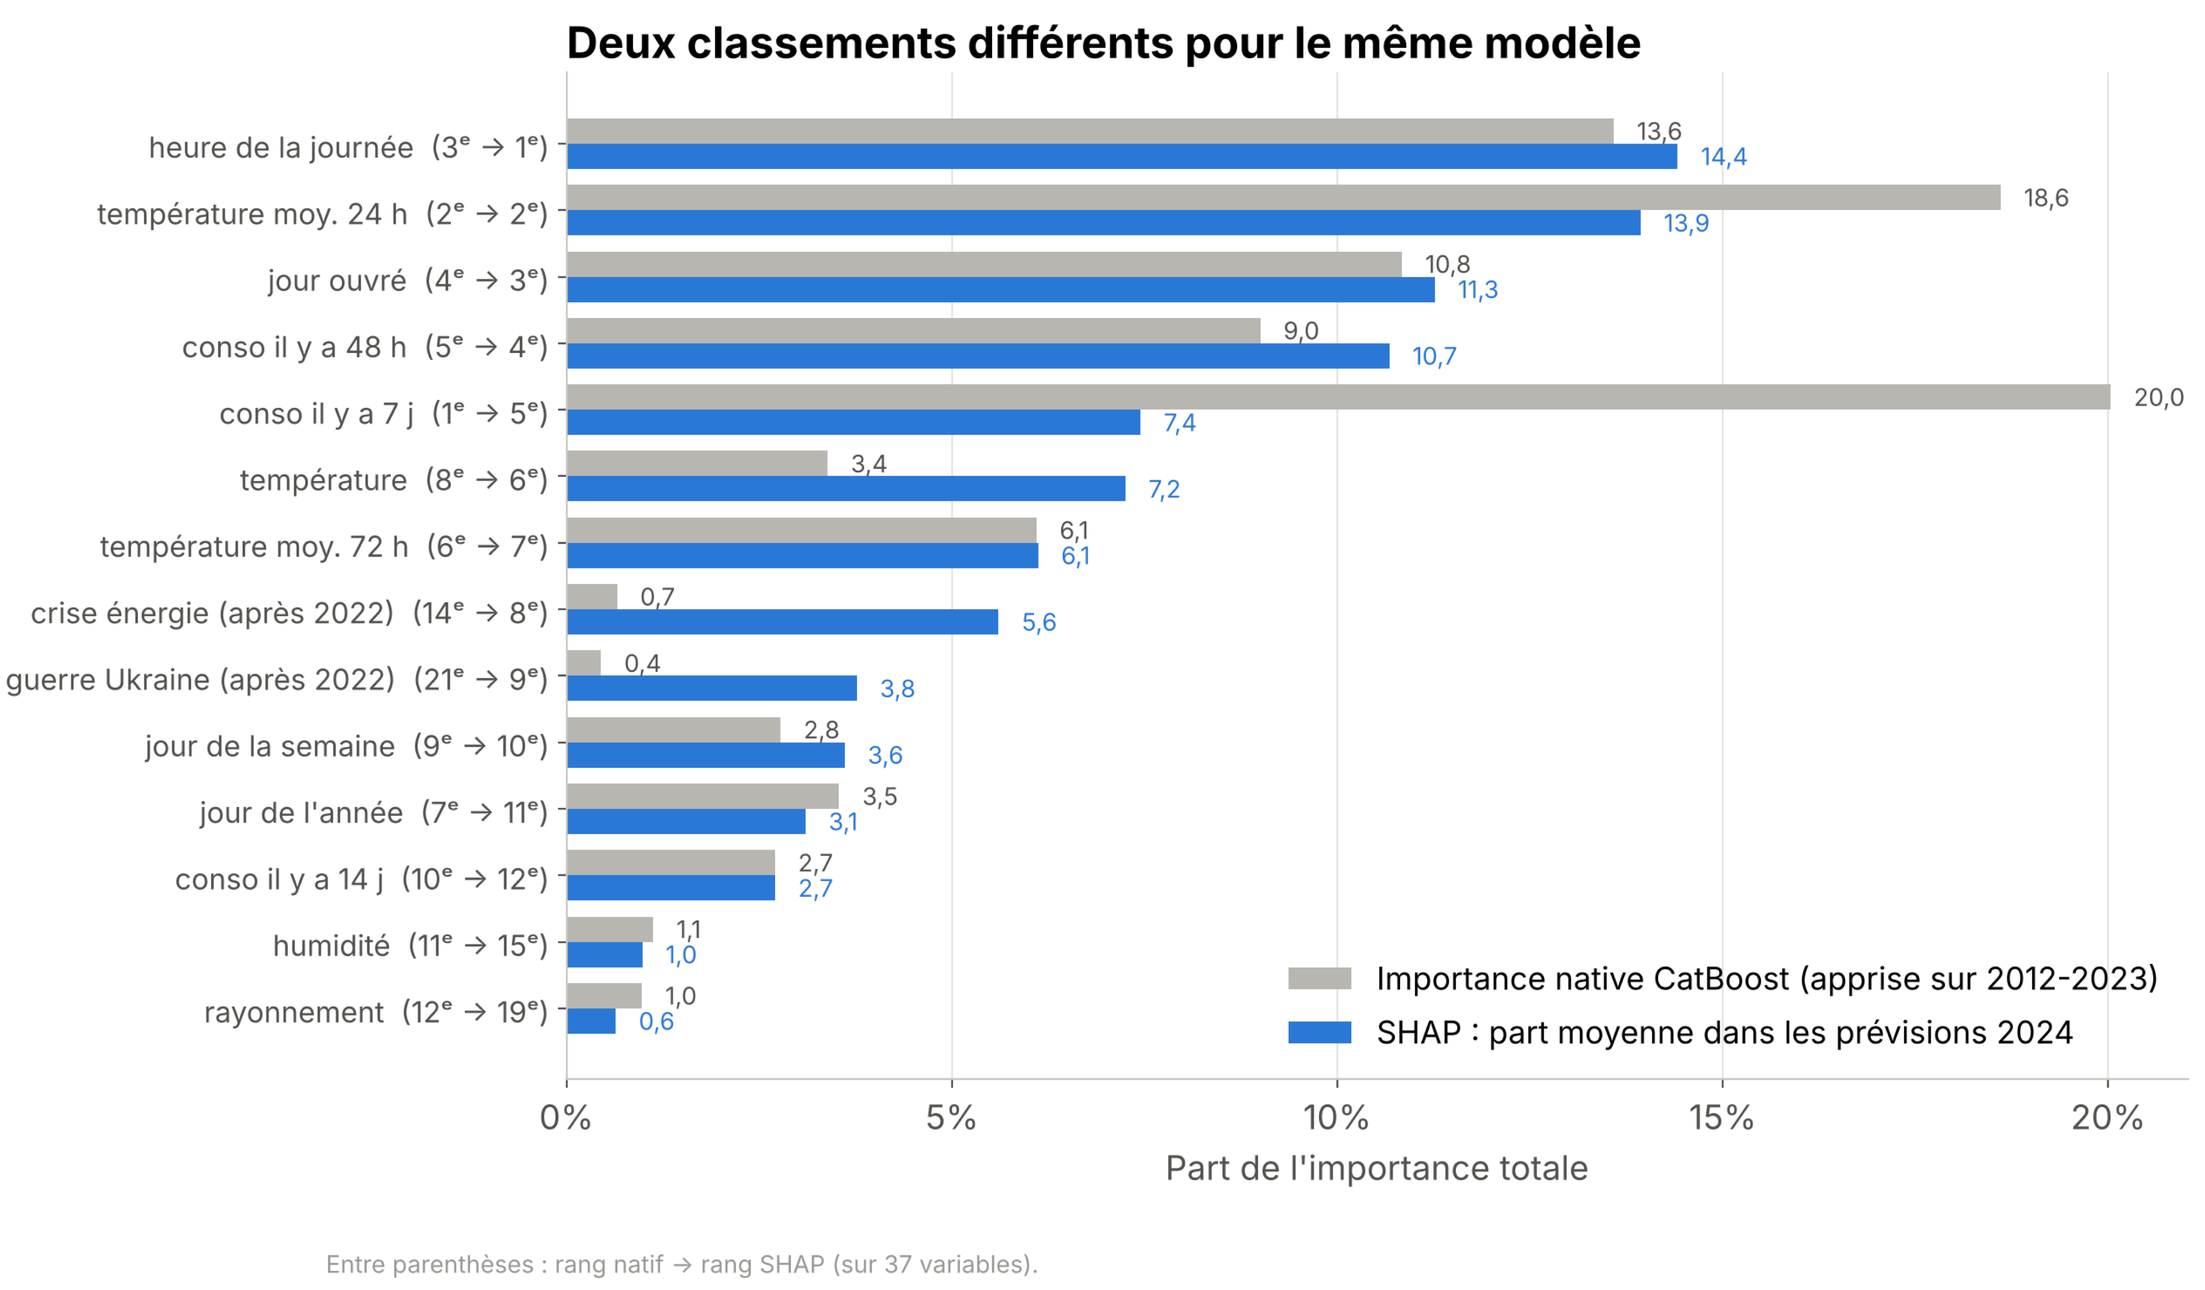
\includegraphics[width=\linewidth]{figures/shap_natif_vs_shap.png}
    \end{column}
    \begin{column}{0.42\textwidth}
      \uncover<2->{%
      \textbf{1. Pas la même question}\\
      Native : où les arbres coupent. SHAP : combien chaque variable pèse dans la prévision.
      Conso il y a 7 jours : \textbf{20 $\to$ 7\,\%}, le mérite est partagé avec le lag 48\,h et la température.}

      \vspace{0.6em}
      \uncover<3->{%
      \textbf{2. Pas les mêmes données}\\
      Native sur 2012-2023, SHAP sur 2024.
      Crise énergie : \textbf{0,7 $\to$ 5,6\,\%}, elle vaut 1 toute l'année 2024.}

      \vspace{0.6em}
      \uncover<4->{%
      \textbf{3. Ce qu'on garde}\\
      Le haut du classement est stable. On retient \textbf{SHAP} pour les trois modèles.}
    \end{column}
  \end{columns}
\end{frame}

% =====================================================================
\begin{frame}{L'apprentissage}
  \begin{columns}[T]
    \begin{column}{0.33\textwidth}\fig{1}{XGBoost}{figures/xgboost_05_apprentissage.png}\end{column}
    \begin{column}{0.33\textwidth}\fig{2}{LightGBM}{figures/lightgbm_05_apprentissage.png}\end{column}
    \begin{column}{0.33\textwidth}\fig{3}{CatBoost}{figures/catboost_05_apprentissage.png}\end{column}
  \end{columns}
  \vspace{0.6em}
  \begin{itemize}
    \item<4-> Arrêt : XGBoost \textbf{702 arbres} (profondeur 7), LightGBM 3\,000, CatBoost 3\,106
    \item<5-> Chez les trois, la validation \textbf{plafonne tôt} alors que l'entraînement continue de baisser : les derniers arbres apprennent par c\oe{}ur
  \end{itemize}
\end{frame}

% =====================================================================
\begin{frame}{Pourquoi on fait mieux que RTE}
  \begin{columns}[T]
    \begin{column}{0.48\textwidth}
      \uncover<1->{%
      \textbf{1. RTE se trompe davantage depuis 2022}
      \begin{itemize}
        \item MAPE $\approx$ 1,5\,\% jusqu'en 2021, 2,86\,\% en 2024
        \item Sous-estimation concentrée à 0\,h, 13-15\,h et 20-21\,h
        \item Corrigé heure par heure, RTE tombe à \textbf{1,69\,\%}
      \end{itemize}}
    \end{column}
    \begin{column}{0.48\textwidth}
      \uncover<2->{%
      \textbf{2. Notre météo est mesurée, pas prévue}
      \begin{itemize}
        \item RTE prévoit avec une température prévue la veille
        \item 1\,$^{\circ}$C d'erreur en hiver $\approx$ 2,4 GW
        \item \alert{Notre avance est donc optimiste}
      \end{itemize}}
    \end{column}
  \end{columns}
  \vspace{1.2em}
  \uncover<3->{%
  \begin{block}{À vérifier ensemble}
    XGBoost annonce une \textbf{météo prévue la veille} : il faut la même météo pour les trois modèles avant de comparer à RTE (diapo suivante).
  \end{block}}
\end{frame}

% =====================================================================
\begin{frame}{Météo : mesurée pour apprendre, prévue pour évaluer}
  En vrai, on ne connaît pas la météo de demain : seulement sa prévision.

  \vspace{1.2em}
  \centering
  \begin{tikzpicture}
    \fill[fondCarte] (0,0) rectangle (9,0.9);
    \node at (4.5,0.45) {\textbf{Entraînement 2012-2023} : météo \textbf{mesurée}};
    \fill[bleuPOWER!80!black] (9,0) rectangle (10.3,0.9);
    \node[text=white,align=center,font=\small] at (9.65,0.45) {Valid\\2024};
    \fill[bleuPOWER] (10.3,0) rectangle (11.6,0.9);
    \node[text=white,align=center,font=\small] at (10.95,0.45) {Test\\2025};
    \draw[bleuPOWER,thick,decorate,decoration={brace,mirror,amplitude=5pt},visible on=<2->] (9,-0.1) -- (11.6,-0.1)
      node[midway,below=6pt,font=\small\bfseries,text=bleuPOWER] {météo prévue la veille};
  \end{tikzpicture}

  \vspace{1.2em}
  \raggedright
  \uncover<3->{%
  \textbf{Contraintes}
  \begin{enumerate}
    \item Météo-France ne publie pas l'archive de ses prévisions
    \item Archive gratuite des prévisions de la veille seulement \textbf{depuis 2024} (Open-Meteo)
    \item Avant 2024 : archive ECMWF réservée à la recherche, très lourde
  \end{enumerate}}

  \vspace{0.4em}
  \uncover<4->{\alert{Les scores LightGBM et CatBoost de cette présentation sont encore en météo mesurée.}}
\end{frame}

% =====================================================================
\begin{frame}{Les difficultés rencontrées}
  \begin{columns}[T]
    \begin{column}{0.46\textwidth}
      \uncover<1->{%
      \textbf{Les données}
      \begin{itemize}
        \item Prévisions météo archivées \textbf{payantes} en grande quantité
        \item Archive gratuite (ECMWF) : \textbf{des semaines de téléchargement}
        \item Tempo absent avant 2014 (fichiers RTE \og tout bleus\fg{})
        \item Base modifiée en cours de route : tout relancer
      \end{itemize}}
    \end{column}
    \begin{column}{0.46\textwidth}
      \uncover<2->{%
      \textbf{LightGBM}
      \begin{itemize}
        \item Colonnes texte refusées : passage en catégories
        \item Entraînement de 12 min (évaluation sur le train), 20\,s sans
        \item Surestimation depuis 2022 : réglée par \texttt{evt\_energie}
        \item Le \emph{gain} trompe : passage à SHAP
        \item Pas d'arrêt avant 3\,000 arbres
      \end{itemize}}
    \end{column}
  \end{columns}
\end{frame}

% =====================================================================
\begin{frame}{La suite}
  \begin{enumerate}
    \setlength{\itemsep}{1em}
    \item<1-> \textbf{Harmoniser} : mêmes variables (\texttt{evt\_energie}, températures lissées), même météo, importance en SHAP
    \item<2-> \textbf{Le froid} : les trois sous-estiment les pics au-dessus de 75 GW
    \item<3-> \textbf{Le sur-apprentissage} : arbres plus simples, validation sur plusieurs années
    \item<4-> \textbf{Le test 2025}, une seule fois, avec le meilleur modèle
  \end{enumerate}
\end{frame}


% =====================================================================
\begin{frame}{Le tableau de bord : architecture}
  \centering
  \begin{tikzpicture}[node distance=1.2cm, fleche/.style={-{Stealth[length=3mm]},thick,bleuPOWER}]
    \node[boite] (nav) {\textbf{Navigateur}\\[0.2em]accès local\\\texttt{127.0.0.1:8501}};
    \node[boite,right=of nav,visible on=<2->] (app) {\textbf{Application}\\[0.2em]\texttt{app.py}\\configuration, navigation};
    \node[boite,right=of app,visible on=<3->] (pages) {\textbf{Trois pages}\\[0.2em]Vue d'ensemble\\Prédictions $\cdot$ Performances};
    \draw[fleche,visible on=<2->] (nav) -- (app);
    \draw[fleche,visible on=<3->] (app) -- (pages);
  \end{tikzpicture}

  \vspace{1.5em}
  \uncover<4->{%
  \begin{tabular}{lll}
    \toprule
    \textbf{Application} & \textbf{Composants} & \textbf{Visualisation} \\
    \midrule
    Python + Streamlit & pages, styles partagés & Plotly + Pandas \\
    \texttt{app.py} & \texttt{pages/}, \texttt{ui.py}, \texttt{styles.css} & graphiques, données \\
    \bottomrule
  \end{tabular}}

  \vspace{1em}
  \uncover<5->{Lancement en local : \texttt{streamlit run app.py}}
\end{frame}

% =====================================================================
\begin{frame}{Le tableau de bord : les trois pages}
  \begin{columns}[T]
    \begin{column}{0.31\textwidth}
      \uncover<1->{%
      \textbf{1. Vue d'ensemble}
      \begin{itemize}
        \item 4 indicateurs : observations, variables, modèle
        \item Évolution de la consommation
        \item Chaîne : données $\to$ préparation $\to$ modèle $\to$ prévision
      \end{itemize}}
    \end{column}
    \begin{column}{0.31\textwidth}
      \uncover<2->{%
      \textbf{2. Prédictions}
      \begin{itemize}
        \item Réglage des paramètres du modèle
        \item Consommation prévue en MW
        \item Comparaison réel / prévu
      \end{itemize}}
    \end{column}
    \begin{column}{0.31\textwidth}
      \uncover<3->{%
      \textbf{3. Performances}
      \begin{itemize}
        \item MAE, RMSE, MAPE
        \item Réel contre prévu (nuage de points)
        \item Répartition des erreurs
      \end{itemize}}
    \end{column}
  \end{columns}
  \vspace{1.5em}
  \uncover<4->{\centering\textbf{Prochaine étape :} y brancher les prévisions des trois modèles et de RTE.\par}
\end{frame}

% =====================================================================
\begin{frame}{À retenir}
  \begin{enumerate}
    \setlength{\itemsep}{1em}
    \item<1-> Les trois modèles \textbf{battent RTE} sur 2024 et se trompent aux mêmes endroits (froid, pics)
    \item<2-> \textbf{CatBoost et LightGBM devant}, grâce à \texttt{evt\_energie} et aux températures lissées
    \item<3-> Avance sur RTE \textbf{en partie optimiste} : météo mesurée et biais de RTE depuis 2022
    \item<4-> Un tableau de bord prêt à accueillir les résultats
  \end{enumerate}
\end{frame}

% =====================================================================
\begin{frame}{Le planning jusqu'à la soutenance}
  \vspace*{-0.6em}
  \centering
  \begin{tikzpicture}[x=0.82cm,y=0.255cm,font=\scriptsize]
    \def\gx{0}
    % mois (semaines : 9/11, 16, 23, 30, 7/12, 14, 21, 28, 4/1, 11, 18, 25)
    \node[anchor=west,text=grisTexte] at (0,1) {nov.};
    \node[anchor=west,text=grisTexte] at (3.3,1) {déc.};
    \node[anchor=west,text=grisTexte] at (7.6,1) {janv.};
    \foreach \s in {0,...,12} \draw[black!12] (\s,0.3) -- (\s,-22.5);
    \draw[bleuPOWER,thick] (0,0.3) -- (12,0.3);
    % une ligne : étape, rang, début, fin, style
    \ggroupe{Données}{0.6}{1}
    \gtache{Base PostgreSQL}{1.6}{0}{0.6}{ganttFait}{1}
    \gtache{Météo, calendrier, prix}{2.6}{0}{0.6}{ganttFait}{1}
    \gtache{Features historiques}{3.6}{0}{2}{ganttFait}{1}
    \gtache{Tempo (testé, retiré)}{4.6}{1}{1.6}{ganttFait}{1}
    \gtache{Encodage de cible}{5.6}{0}{2.3}{ganttCours}{1}
    \gtache{Météo prévue (Open-Meteo)}{6.6}{2}{5}{ganttVenir}{1}
    \ggroupe{Analyses exploratoires}{7.8}{2}
    \gtache{Corrélations}{8.8}{1}{3}{ganttVenir}{2}
    \gtache{Distribution, variance}{9.8}{1}{4}{ganttVenir}{2}
    \gtache{Valeurs extrêmes (Pareto)}{10.8}{2}{5}{ganttVenir}{2}
    \ggroupe{Modèles}{12}{3}
    \gtache{Tests des trois modèles}{13}{0}{5}{ganttCours}{3}
    \gtache{Importance (SHAP)}{14}{1}{7}{ganttCours}{3}
    \gtache{Analyse des erreurs}{15}{1}{8}{ganttCours}{3}
    \gtache{Optimisation}{16}{7}{10}{ganttVenir}{3}
    \gtache{Test final 2025 (une fois)}{17}{10}{11}{ganttVenir}{3}
    \ggroupe{Livrables}{18.2}{4}
    \gtache{Dashboard}{19.2}{0}{11}{ganttCours}{4}
    \gtache{Rapport (au fil de l'eau)}{20.2}{0}{11}{ganttCours}{4}
    \node[anchor=west,visible on=<4->] at (-4.8,-21.2) {Comité d'organisation};
    \fill[ganttJalon,visible on=<4->] (5,-21.2) +(0,0.5) -- +(0.2,0) -- +(0,-0.5) -- +(-0.2,0) -- cycle;
    \node[anchor=west,visible on=<4->] at (-4.8,-22.2) {Soutenance};
    \fill[ganttJalon,visible on=<4->] (12,-22.2) +(0,0.5) -- +(0.2,0) -- +(0,-0.5) -- +(-0.2,0) -- cycle;
    % aujourd'hui : mercredi 18 novembre
    \draw[orangeRTE,very thick,dashed,visible on=<5->] (1.3,0.3) -- (1.3,-22.6);
    \node[text=orangeRTE,font=\scriptsize\bfseries,anchor=west,visible on=<5->] at (1.35,-7.8) {aujourd'hui, 18 nov.};
    % légende
    \begin{scope}[shift={(0,-24)}]
      \fill[ganttFait] (0,-0.35) rectangle (0.5,0.35);  \node[anchor=west] at (0.55,0) {terminé};
      \fill[ganttCours] (2.6,-0.35) rectangle (3.1,0.35); \node[anchor=west] at (3.15,0) {en cours};
      \fill[ganttVenir] (5.2,-0.35) rectangle (5.7,0.35); \node[anchor=west] at (5.75,0) {à venir};
      \fill[ganttJalon] (8.05,0) +(0,0.5) -- +(0.2,0) -- +(0,-0.5) -- +(-0.2,0) -- cycle; \node[anchor=west] at (8.3,0) {jalon};
    \end{scope}
  \end{tikzpicture}
\end{frame}

\end{document}
